\documentclass{article}
\usepackage[utf8]{inputenc}
\usepackage{listings}
\usepackage[spanish]{babel}
\usepackage{graphicx}
\usepackage{minted}
\usepackage{xcolor}


\newminted{bash}{
    style=monokai,
    bgcolor=monokaibg
}

\BeforeBeginEnvironment{bashcode}{\color{monokaifg}}
\AfterEndEnvironment{bashcode}{\color{black}}

\title{Conservation Genomics Tarea 01}
\author{Angel Luis Robles Fernandez}
\date{September 2020}



\begin{document}

\maketitle

\section{Introduction}

A partir de archivos de lecturas rápidas de secuencia (RadSeq) es posible obtener los $SNB_s$. Estos $SNB_s$ permiten estimar estadísticos sobre la población de la cuál se tomaron las muestras y conocer mejor su estructura.


\section{Métodos}

Primero creamos una carpeta  nueva para el proyecto y copiamos los archivos de dummy\_raw\_reads.
\begin{minted}[bgcolor=black,mathescape=false, formatcom=\color{white}]{bash}
        [usuario@equipo] $ makedir ref_map
\end{minted}

\begin{minted}[bgcolor=black,formatcom=\color{white}]{bash}
        usuario@equipo $ makedir /ref_map/dummy_raw_reads
\end{minted}

\begin{minted}[bgcolor=black,formatcom=\color{white}]{bash}
usuario@equipo $ process_radtags -i gzfastq 
-p ./dummy_raw_reads/
-o ./samples_output/
-b ./info/barcodes_lane1.txt
-e pstI -r -c -q -D -s 30
\end{minted}

Esto genera en la carpeta samples\_output los archivos fastq necesarios para el alineamiento.

Posteriormente se utiliza bwa para indexar el genoma de referencia:

\begin{minted}[bgcolor=black,formatcom=\color{white}]{bash}
usuario@equipo $ bwa index assembly_scaffolds.fasta
\end{minted}

Al tener varios archivos fastq como salid de los radtags procesados se utiliza un script de bash para generar los archivos bam. Utilizando el manual de stacks, Catcher sugiere el siguiente pipline:

\begin{minted}[bgcolor=white,formatcom=\color{black}]{bash}

#!/bin/bash
src=$HOME//conservationGenomics/stacks/taller2/ref_map

files="
Lco012
bLco02
bLco020
bLco021
bLco024
bLco027
bLco030
bLco031
bLco038
bLco09
bLco302
bLco312
bLco313
bLco315
bLco316
bLco320
bPon_461
bPon020
bPon048
bPon078
bPon084
bPon085
bPon167
bPon320
bPon338
bPon344
bPon353
bPon367
bPon376
bPon377
bPon392
bPon393
bPon404
bPon406
bPon409
bPon423
bPon430
bPon441
bPon446
bPon453
bPon460
bPon461
bPon477
F12
F14
F30
F348
F398400
F415
F427
F429
"

#
# Align paired-end data with BWA, convert to BAM and SORT.
#

for sample in $files
do
    bwa mem -t 8 
    assembly_scaffolds.fasta $src/samples_output/${sample}.fq.gz |
      samtools view -b |
      samtools sort --threads 4 > $src/aligned/${sample}.bam
done
\end{minted}

Hacemos ejecutable el script con:


\begin{minted}[bgcolor=black,formatcom=\color{white}]{bash}
usuario@equipo $ chmod -x script.sh
\end{minted}


Posteriormente podemos utilizar el wraper ref\_map.pl para correr gstacks y populations 


\begin{minted}[bgcolor=black,formatcom=\color{white}]{bash}
usuario@equipo $ ref_map.pl
--samples ./aligned
--popmap ./info/pop_map_25smp.txt
-o ./results/stacks -T 4
\end{minted}
 
 Finalmente utilizamos populations para generar un vcf

\begin{minted}[bgcolor=black,formatcom=\color{white}]{bash}
usuario@equipo $ populations 
-P ./results/stacks  
--popmap ./info/pop_map_25smp.txt 
--write-single-snp  
--vcf -O ./results
\end{minted}





\section{Resultados}

A continuación se presenta una tabla con el resumen estadístico por población

\begin{table}[]
\begin{tabular}{ccccccl}
pop\_id & p     & pi    & obs\_hom & exp\_het & fis   &  \\ \cline{1-6}
ama     & 0.769 & 0.332 & 0.751    & 0.26     & 0.184 &  \\
atl     & 0.822 & 0.174 & 0.853    & 0.103    & 0.043 &  \\
cat     & 0.827 & 0.151 & 0.859    & 0.087    & 0.014 &  \\
cer     & 0.818 & 0.202 & 0.832    & 0.125    & 0.055 &  \\
pan     & 0.793 & 0.288 & 0.789    & 0.221    & 0.172 & 
\end{tabular}
\end{table}



Se anexa un gráfico (\ref{fig:fig1})  de los haplotipos por población con respecto al \textit{locus}, agrupado por cada población generado en R.

\begin{figure}[h]
    \centering
    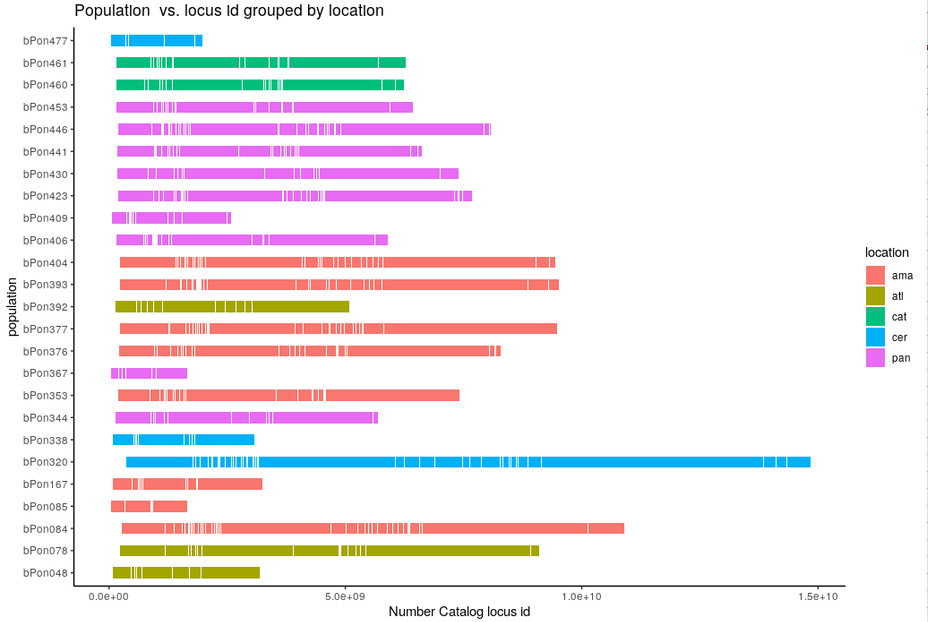
\includegraphics[width=1.5\textwidth]{haplotypes_1.png}
    \caption{Population vs locus id grouped by location}
    \label{fig:fig1}
\end{figure}

\end{document}
